\documentclass[a4paper,10pt]{article}

\newcommand{\blatt}{12}
\newcommand{\autor}{Merlin Steuer, Till Schander}

\usepackage{hci}
\usepackage{graphicx}
\usepackage{caption}
\usepackage{subcaption}
\usepackage{enumerate}

\begin{document}
% Seitenkopf mit Informationen
\kopf
\renewcommand{\figurename}{Figure}

\aufgabe{17}

Entwickelt werden soll eine Smartwatch-App, welche es innerhalb einer Smart-Home-Umgebung erlaubt, die Temperatur und Qualität der Luft zu überwachen und zu manipulieren. Überwachte Parameter sind u.a. die Temperatur, die Luftfeuchtigkeit, der Sauerstoffgehalt sowie ggf. Schadstoffgehalt in der Raumluft. Mittels der App sollen mit einfachen Befehlen Belüftungs- und Heizsysteme gesteuert werden können.

\tableofcontents

\newpage



\section{Analyse}

\subsection{PACT-Analyse}

\begin{itemize}
    \item Persons: 
        \begin{itemize}
            \item Junge Eigenheimbesitzer
            \item 25-45 Jahre alt
            \item Technikinteressiert und -affin
            \item Besitzer von Smartwatches auf Android- oder iOS-Basis
            \item Besitzer eines vollausgestatteten Smart-Homes
        \end{itemize}
    \item Activities:
        \begin{itemize}
            \item Überwachen der Raumtemperatur
            \item Überwachen der Luftfeuchtigkeit
            \item Überwachen des Sauerstoff- und Schafstoffgehalts der Raumluft
            \item Anzeige eines aggregierten Werts für die Luftqualität
            \item Manipulieren der Umgebungsluft durch Steuerung verschiedener Belüftungs-, Luftbefeuchtungs- und Heizanlagen
            \item Einstellung von Automatismen zum Erhalt einer stabilen Luftqualität
        \end{itemize}
    \item Context:
        \begin{itemize}
            \item Das eigene Heim
            \item Übliche Aufenthaltsorte wie Schlafzimmer und Wohnzimmer. Weniger Augenmerk auf Küche oder Bad
            \item Besondere Nutzung während der Abendstunden zur gemütlichen Zeit
            \item Ggf. für Home-Office-Arbeiter zur Erhaltung einer stabilen Luftqualität bei der Arbeit (Einstellung am PC/Smartphone, Ansteuerung per Smart-Watch)
        \end{itemize}
    \item Technologies:
        \begin{itemize}
            \item Smart-Watch (Android oder iOS) als Steuerungssystem
            \item Diverse Sensoren zum Erfassen der relevanten Luftinformationen
            \item Ein Smart-Home System auf XBee oder ZWave-Basis, welches leicht durch Drittanbieter zu erweitern ist.
        \end{itemize}
\end{itemize}

\newpage



\subsection{Szenarien}

\subsubsection{Szenario 1}
Peter Klein kommt nach der Arbeit gegen 19 Uhr nach Hause in seine 3-Zimmer Wohnung in der Innenstadt einer großen Metropole. Er empfindet die Luft in seiner Wohnung wegen der exponierten Dachgeschosslage als sehr trocken und heiß.

Um etwas dagegen zu unternehmen schaltet Peter die Klimaanlage seiner Wohnung ein und stellt den Raumluftbefeuchter im Wohnzimmer auf maximale Stufe.

Bevor er ins Bett geht schaltet Peter die Geräte wieder aus um Strom zu sparen und die Lärmbelästigung zu reduzieren.

\subsubsection{Szenario 2}
Annemarie Groß ist Mutter von drei Schulkondern im Grundschulalter. Ihre Kinder haben oft Konzentrationsprobleme, weshalb Sie einen Spezialisten um Hilfe bat, welcher Ihre Luftqualität in der Wohnung bemängelte.

Die Kinder kommen gegen frühen Nachmittag nach Hause. Da Annemarie vormittags daheim ist überprüft Sie mittels diverser Messgeräte die Luftqualität und nimmt entsprechend der Messwerte verschiedene Aktionen in Angriff. Heute ist der Sauerstoffgehalt sehr schlecht und die Schadstoffbelastung hochm, also schaltet Annemarie einen Raumluftionisierer zur Reinigung von Schadstoffen ein und erhöht mittels eines speziellen Apparates den Sauerstoffgehalt der Luft von 16,7 auf 17,1 Prozent.

Seit diese Maßnahmen durchgeführt werden haben Annemaries Kinder deutlich weniger Konzentrationsschwierigkeiten.

\newpage



\section{Design}

\subsection{Icon}

\begin{figure}[!h]
	\centering
	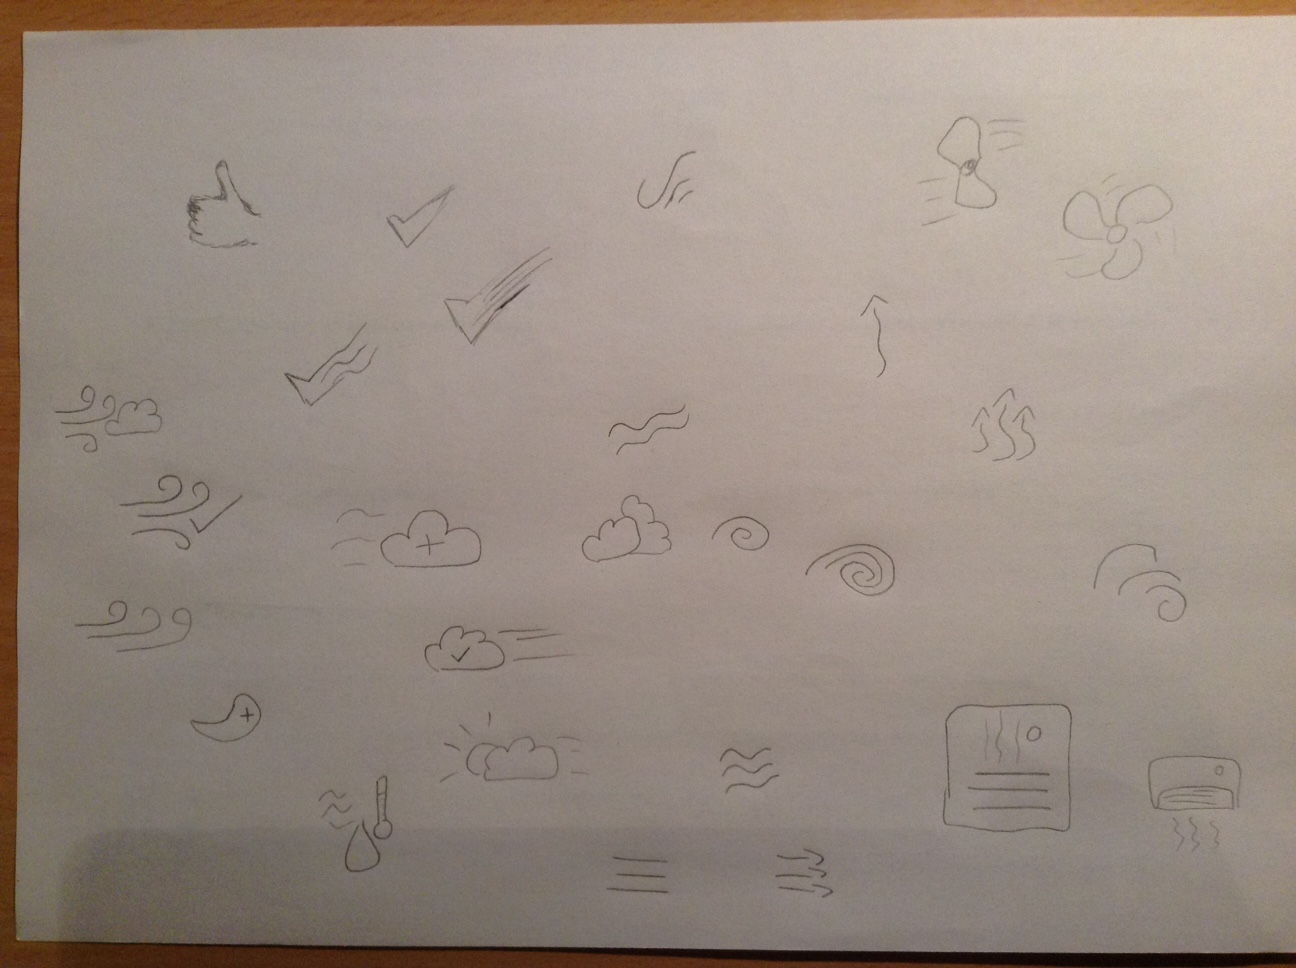
\includegraphics[scale=0.3]{images/sketches1.jpg}
	\caption{Verschiedene Optionen des Logos}
\end{figure}

Da der Focus der Anwendung auf der Luftqualität liegt, wurde versucht Luft möglichst verständlich in dem Icon abzubilden. Dies wird dadurch erschwert, dass Luft an sich durchsichtig ist.

Eine Option die erkundet wurde, ist das Abbilden von Wolken. Da Wolken Gase in der Luft sind (meistens Wasserdampf), war dies eine relativ passende Metapher für unsere Anwendung. Insbesondere die Verbindung zu Wasserdampf ist optimal, da auch die Steuerung der Luftfeuchtigkeit mit der Anwendung möglich ist. Allerdings stellte sich schnell heraus, dass Wolken vor allem als Icon für das Wetter gesehen werden. Somit bestünde also eine große Verwechslungsgefahr mit Wetteranwendungen. Dieser Ansatz wurde daher nicht gewählt.

Eine weitere Option war das Abbilden einer Klimaanlage. Weil Klimaanlagen jedoch meist, unscheinbare Kästen sind, war es schwer diese in als Icon darzustellen. Hier bestand Verwechslungsgefahr mit anderen Haushaltsgeräten wie beispielsweise Öfen.

Ein relativ weit verbreitetes Bild von Luft ist sind verwirbelte Striche, welche Wind nachbilden. Damit diese Wirbel nicht mit Wasser verwechselt werden, haben wir uns gegen Wellen und für relativ lange Striche mit kleinen Wirbeln am Ende entschieden. Um zusätzlich den Aspekt der Qualität mit einzubeziehen, wurde eine Ausgestreckter Daumen in Betracht gezogen. Dieser wurde jedoch durch den geometrisch simpleren Haken ersetzt. Kombiniert ergeben diese beiden Elemente unser Logo.

\newpage



\subsection{Prototyp}

\begin{figure}[!h]
	\centering
	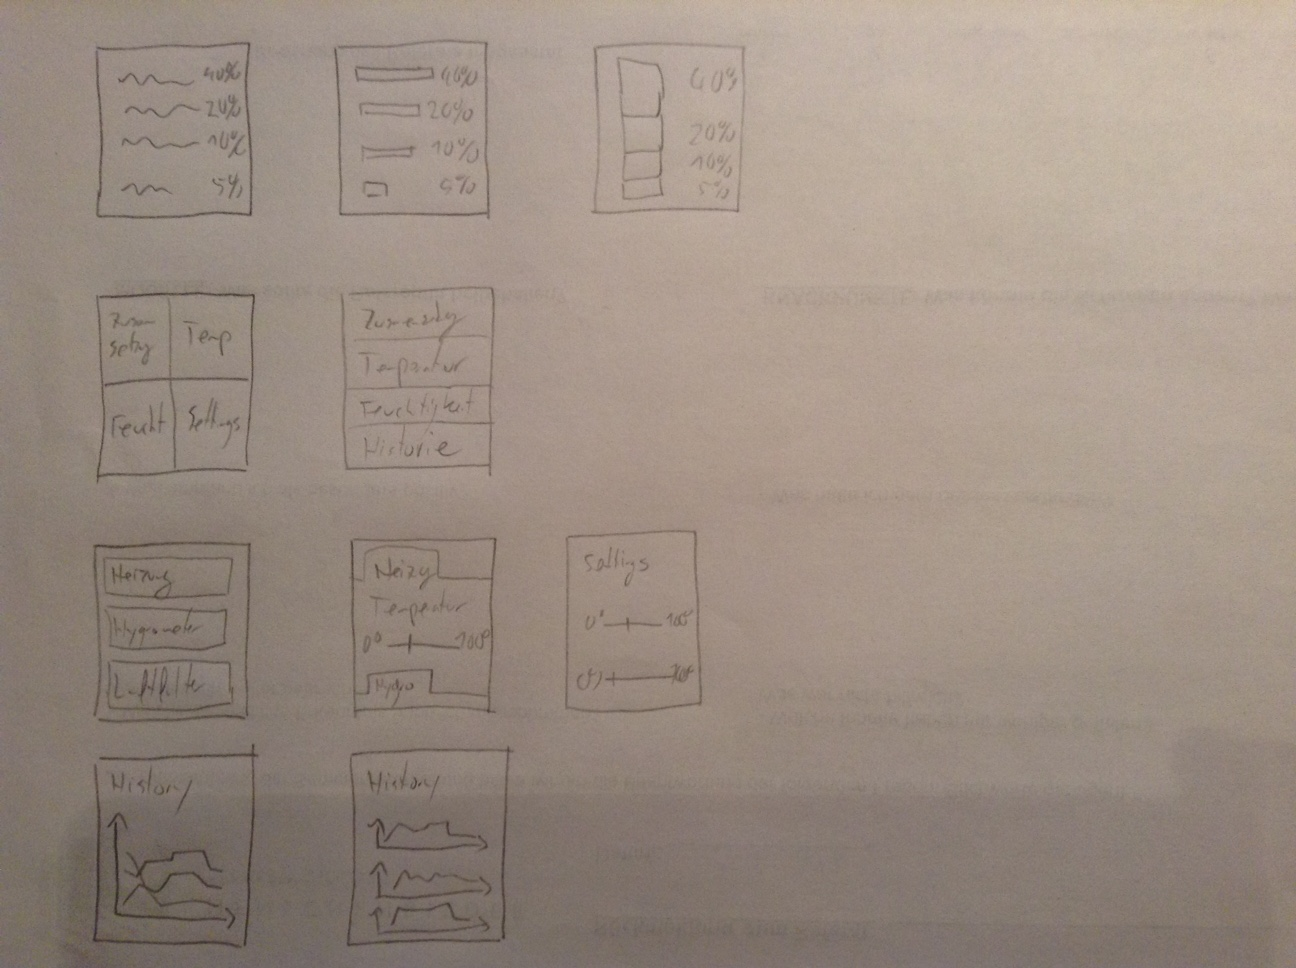
\includegraphics[scale=0.3]{images/sketches2.jpg}
	\caption{Sketches der Anwendung}
\end{figure}

Aus der PACT-Analyse und den Szenarien war relativ schnell klar, was die Anwendung können soll. Zentrales Element ist die Zusammensetzung der Luft. Aus welchen Bestandteilen die Luft aktuell besteht soll prozentual aufgeschlüsselt werden. Dazu sollen die einzelnen Bestandteile grafisch dargestellt werden. Anfangs wurde dies mit einem Balkendiagramm gemacht, aus Platzgründen haben wir uns jedoch für nur einen Balken entschieden.

Eine weiter zentrale Funktionalität der Anwendung ist das Aktivieren verschiedener Geräte, wie z.B. der Heizung. Hierfür war anfangs ein Knopf für jedes Gerät vorgesehen. Diese Knöpfe befanden sich untereinander in einer Liste. Da jedoch bestimmte Parameter, wie die Temperatur, nicht mit einem einfachen Knopf einzustellen sind, haben wir uns dafür entschieden, die einzelnen Geräte und ihre Bedienelemente separat anzuzeigen.

Vergangene Messwerte sollen auch einsehbar sein, um aktuelle Werte in Relation setzen zu können. Aus Platzgründen wurden diese Werte anfangs in nur einen Diagramm abgebildet. Da jedoch, je nach Wert, unterschiedliche Einheiten verwendet werden, ergab dies wenig Sinn. Nun werden daher mehrere, wenn auch kleine, Graphen verwendet.

Die einzelnen Funktionen können von einem Startbildschirm aus angewählt werden. Dieser ist ziemlich schlicht und bietet mit großen Flächen einfache Ziele zum Auswählen.

\newpage



\section{Implementierung}

\subsection{Icon}

\begin{figure}[!h]
	\centering
	
\includegraphics[scale=0.4]{images/logo.png}
	\caption{Das Icon der Anwendung}
\end{figure}

Das Icon ist möglichst simpel gehalten, aber nicht zu simpel, damit es gut im Gedächtnis bleibt (Gesetz der guten Gestalt). Es besteht aus einem Wind von links, der auf einen Haken trifft. Somit soll die Luftqualität symbolisiert werden. Die Farben Blau und Weiß finden sich so auch in der Luft am Himmel wieder. Außerdem wurden sie auch in der Anwendung verwendet, was ein stimmiges Gesamtbild abgibt. Der leichte Verlauf im Hintergrund ist vorhanden, da das Icon ohne ihn zu simpel, gar langweilig, ausgesehen hätte.

Die drei Striche der Luft werden aufgrund ihrer Nähe als zusammengehörig wahrgenommen (Gesetz der Nähe und Gesetz des gemeinsamen Schicksals). Die Luft scheint auf den Haken zu treffen, prallt jedoch von diesem ab. Dies kann symbolisch dafür verstanden werden, dass die Luftqualität konstant gut bleibt. Da die beiden Elemente Luft und Haken ungefähr gleich viel Platz einnehmen, bildet sich ein harmonisches Gleichgewicht.

\newpage



\subsection{Prototyp}

\begin{figure}[!h]
    \centering
    
    \begin{subfigure}[!h]{0.3\textwidth}
        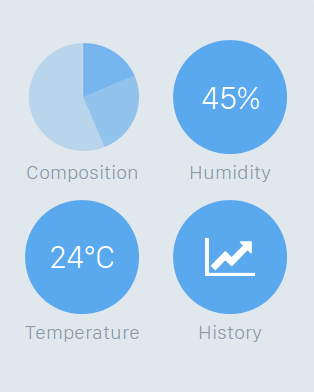
\includegraphics[width=\textwidth]{images/home.png}
        \caption{Home}
    \end{subfigure}
    \begin{subfigure}[!h]{0.3\textwidth}
        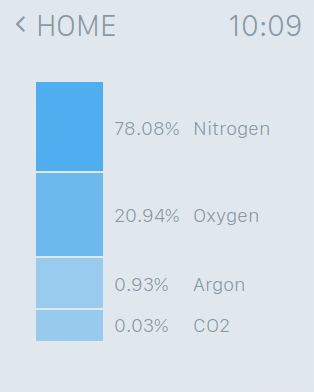
\includegraphics[width=\textwidth]{images/composition.png}
        \caption{Composition}
    \end{subfigure}
    \begin{subfigure}[!h]{0.3\textwidth}
        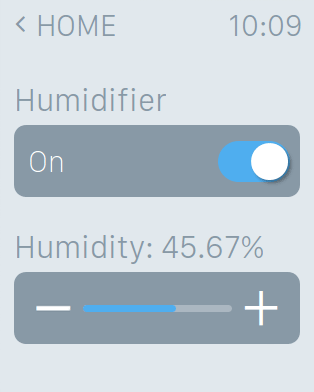
\includegraphics[width=\textwidth]{images/humidity.png}
        \caption{Humidity}
    \end{subfigure}
    
    \begin{subfigure}[!h]{0.3\textwidth}
        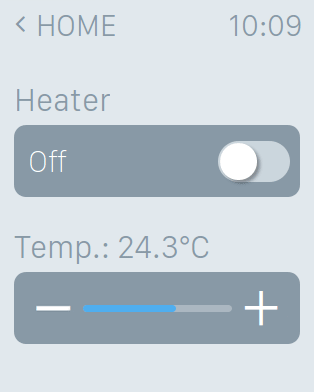
\includegraphics[width=\textwidth]{images/temperature.png}
        \caption{Temperature}
    \end{subfigure}
    \begin{subfigure}[!h]{0.3\textwidth}
        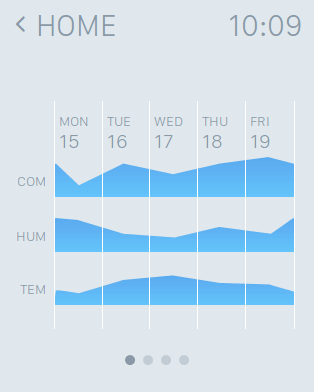
\includegraphics[width=\textwidth]{images/history.png}
        \caption{History}
    \end{subfigure}
    
    \caption{Die einzelnen Screens des Prototypen}
\end{figure}

Für die Erstellung der Screens wurde die Axure-Vorlage aus OLAT verwendet. Bestimmte Elemente wie Schalter und Slider waren somit in ihrer Form vorgegeben. Auch das Farbschema stammt aus dieser Vorlage, ist wie unter 3.1 beschrieben jedoch sehr passend für diese Anwendung.

Die Einstiegsseite besteht aus vier großen Kreisen. Diese bilden aufgrund ihrer Größe gute Klickflächen. Des weiteren werden erste Informationen schon hier angezeigt. Um die aktuelle Luftfeuchtigkeit zu sehen muss also keine Unterseite angewählt werden. Dies ist maximal effizient.

Der obere Bereich ist auf allen Unterseiten gleich. Am linken Rand befindet sich ein Escape-Hatch, um zurück auf die Einstiegsseite zu gelangen und rechts wird die Uhrzeit angezeigt. Diese Regelmäßigkeit lässt alle Seiten vertraut und einheitlich aussehen, wodurch sich Nutzer schneller zurecht finden und die Anwendung insgesamt ``runder'' wirkt. 

Die Bedienelemente für Luftbefeuchter und Heizung sind sehr groß, sodass sie auch mit dickeren Fingern noch verwendet werden können. Lediglich die Historien-Ansicht ist etwas klein, allerdings gibt es hier auch keine weiteren klickbaren Flächen. Es kann nur die gesamte Ansicht umgeblättert werden, um weitere Tage anzuzeigen. Somit schadet die Kleinteiligkeit nicht der Bedienbarkeit, sondern nur dem Lesekomfort.

\newpage



\section{Evaluation}

Da für die Wahl des Icons mehrere Varianten zur Verfügung standen (siehe 2.1) wurden mehrere ausgeschlossene Optionen in einer Evaluation geprüft. Dazu mussten die Versuchspersonen mehrere Aussagen auf einer Skala von eins bis fünf beantworten. Fünf bedeutete Dabei ``Stimme ich voll zu'' und eins ``Stimme ich überhaupt nicht zu''. Die beiden zu einander gehörenden Fragen (I und II, sowie III und IV) wurden dann mit einem T-Test auf ihre Signifikanz hin untersucht.\\ \\

Die Aussagen lauteten:

\begin{enumerate}[I]

\item
Eine Wolke symbolisiert für mich Luft.

\item
Wellen symbolisieren für mich Luft.

\item
Ein Daumen symbolisiert für mich Qualität.

\item
Ein Haken symbolisiert für mich Qualität. \\

\end{enumerate}

Dies waren die Ergebnisse:\\

\begin{tabular}{c|c|c|c|c|c|c}
& Teilnehmer 1 & Teilnehmer 2 & Teilnehmer 3 & Teilnehmer 4 & Teilnehmer 5 & Teilnehmer 6 \\ 
\hline I   & 2 & 1 & 3 & 2 & 4 & 3 \\ 
\hline II  & 3 & 2 & 1 & 2 & 3 & 3 \\ 
\hline III & 3 & 4 & 3 & 2 & 3 & 4 \\ 
\hline IV  & 5 & 3 & 4 & 4 & 4 & 5 \\
\end{tabular}\\ \\ \\

Für Aussage I und II ist der P-Wert 0.7654. Für Aussage III und IV ist der P-Wert 0.04419. Der Unterschied von Wolke und Wellen (Aussage I und II) ist also nicht signifikant. Somit ist möglicherweise das Symbol auf dem Icon nicht ideal gewählt. Zumindest hätte eine Wolke genau so gut verwendet werden können. Der Unterschied von Daumen und Haken ist hingegen signifikant. Die Versuchsteilnehmer fanden einen Haken einleuchtender. Somit ist dieser Teil des Logos sinnvoll gewählt.\\

Mit nur sechs Teilnehmer ist die Zahl der gewonnen Werte allerdings relativ klein. Es kann sein, dass bei einer anderen Stichprobe ein anderes Ergebnis herausgekommen wäre. Außerdem ist der Versuchsaufbau nicht ideal, da den Teilnehmern keine Grafiken gezeigt wurden. Was sich Versuchsteilnehmer beispielsweise unter  Wellen vorstellen kann somit ganz anders sein, als die Wellen in unserem Icon. Der Versuch sollte also in der Zukunft noch einmal mit Grafiken und mehr Teilnehmern wiederholt werden.

\end{document}
